\section{Security Architectures}\label{sec:Security_Architectures}
\begin{questions}
\question{} Describe what constitutes a security architecture and give some examples.
  \begin{solution}
    A Security Architecture has graphical and textual representations of a security system.
    It includes relations, trust levels, trust relationships, and interfaces between different parts of the system.
    It also has security and system boundaries to delimit different parts of the system that have various properties.
  \end{solution}

\question{} The Sherwood Applied Business Security Architecture (SABSA) consist of 5 layers and one cross layer.
  \begin{parts}
  \part{} Describe the different layer views and list the names of the different layers.
    \begin{solution}
      \begin{enumerate}[noitemsep]
      \item Contextual Security Architecture is the view the business has of the system.
        It is quite similar to the Security Requirements.
      \item Conceptual Security Architecture is the highest-level view that an engineer can have of the system.
        This includes the general breakdown into secure portions of a system.
      \item Logical Security Architecture is the next level, that deals with data and its logical flows.
        Here, the way that data and its logical propagation are safeguarded is first developed.
      \item Physical Security Architecture is the 3rd design level.
        Here, the specific high-level security requirements and previous security architecture levels are combined to choose what needs to be done to secure the data.
      \item Component Security Architecture is the lowest level of the SABSA Security Architecture.
        Here, the actual protocols, standards, and hardware are chosen.
      \item Security Service Management Architecture is the ``cross layer''.
        It is concerned with how to maintain the system and its security.
      \end{enumerate}
    \end{solution}

  \part{} Give examples of questions the different SABSA architecture views are supposed to answer.
    \begin{solution}
      \begin{enumerate}[noitemsep]
      \item Contextual Security Architecture
        \begin{itemize}[noitemsep]
        \item What does the business need from the system?
        \item Why do we need to mitigate against these risks and threats?
        \item How do we protect the processes in this system?
        \item Who are going to be the ones using the system?
        \item Where is this system going to be geographically located and where is this product going to be used?
        \item When does the client require this system and for how long?
        \end{itemize}
      \item Conceptual Security Architecture
        \begin{itemize}[noitemsep]
        \item What does the client need to have protected?
        \item Why are these risks that need to be mitigated and do these assets need protection?
        \item How do we provide protection, in very high-level technical and maanagement security terms/strategies?
        \item Who are the people/organizations involved in the security management and the assumed trust relationships?
        \item Where is protection needed in terms of security domains?
        \item When is the relevant time scope(s) of the system's protection?
        \end{itemize}
      \item Logical Security Architecture
        \begin{itemize}[noitemsep]
        \item What is the actual information being secured?
        \item Why shall this security policy be applied to the system?
        \item How are the actual security services in the system put together?
        \item Who are the entities in the system and how can they interact?
        \item Where are the security domains and the relationships between the domains?
        \item When is the security processing cycle?
        \end{itemize}
      \item Physical Security Architecture
        \begin{itemize}[noitemsep]
        \item What is the data model and security-related data structures?
        \item Why are these the rules that drive logical decisions in the system?
        \item How do these security mechanisms work to provice security and what physical machines or modules are needed?
        \item Who are the users, the applications they use, and the security interface?
        \item Where is the required security infrastructure required to provide the security?
        \item When is the dependency in the system present in the form of execution control structures?
        \end{itemize}
      \item Component Security Architecture
        \begin{itemize}[noitemsep]
        \item What are the data field specifications, address specifications, etc.
        \item Why are we using these security standards and best practices?
        \item How are the entities/modules, tools, etc.\ used and put together?
        \item Who are the users' identities, privileges, functions, actions, Access Control Lists?
        \item Where are the computing processes, nodes addresses, and inter-process protocols?
        \item When are the security step timings and sequencing?
        \end{itemize}
      \item Security Service Management Architecture
        \begin{itemize}[noitemsep]
        \item What is the operational continuity and information processing of the system?
        \item Why do we need to minimize operational risks and mitigate failures/disruptions?
        \item How do we perform these specialized security-related operations?
        \item Who do we support? All users and their applications?
        \item Where do we perform maintainance from and on?
        \item When do we schedule things and execute our time-table of security-related operations?
        \end{itemize}
      \end{enumerate}
    \end{solution}
  \end{parts}

\question{} Which are the three different types of security services in a logical security architecture?
  \begin{solution}
    \begin{enumerate}[noitemsep]
    \item Prevention services
    \item Detection, Notification, Assurance, and Event Collection services
    \item Recovery and Restoration services
    \end{enumerate}
  \end{solution}

  \begin{parts}
  \part{} List and explain examples of services part of the non-prevention type of security services.
    \begin{solution}
      \begin{itemize}[noitemsep]
      \item Detection, Notification, Assurance, and Event Collection services
        \begin{itemize}[noitemsep]
        \item Log review
        \item Message integrity verification
        \item Security monitoring
        \item Audit trails
        \item Security Training/awareness
        \item Intrusion Detection
        \end{itemize}
      \item Recovery and Restoration services
        \begin{itemize}[noitemsep]
        \item Incident response
        \item Data replication
        \item Data backup
        \item Disaster recovery
        \item Crisis management
        \end{itemize}
      \end{itemize}
    \end{solution}
  \end{parts}

\question{} Describe each of the different prevention security services in more details.
  \begin{parts}
  \part{} Give example of at least four different Entity Security Services and how they contribute to security prevention.
    \begin{solution}
      \begin{enumerate}[noitemsep]
      \item Unique Entity naming
      \item Entity registration
      \item Entity credentials certifications
      \item Directory services
      \item Entity authorization
      \item User authentication
      \item Device authentication
      \end{enumerate}
    \end{solution}

  \part{} Give example of at least four different Communication Security Services and how they contribute to security prevention.
    \begin{solution}
      \begin{enumerate}[noitemsep]
      \item Session authentication
      \item Message origin authentication
      \item Non-repudiation
      \item Message reply protection
      \item Traffic flow confidentiality
      \item Security administration
      \item User support
      \item Physical security services
      \item Environmental security services
      \end{enumerate}
    \end{solution}

  \part{} Give example of at least four different Application-level Security Services and how they contribute to security prevention.
    \begin{solution}
      \begin{enumerate}[noitemsep]
      \item Entity authorization
      \item Logical access control
      \item Audit trails
      \item Stored data integrity protection
      \item Stored data confidentiality
      \item Software integrity protection
      \item Software licensing management
      \item System config protection
      \item Data replication
      \item Data backups
      \item Software replication
      \item Software backups
      \item Trusted time
      \item Secure user interface
      \end{enumerate}
    \end{solution}

  \part{} Give example of at least four Security Management Services and how they contribute to security prevention.
    \begin{solution}
      \begin{enumerate}[noitemsep]
      \item Security policy management
      \item Security training and awareness
      \item Security ops management
      \item Security provisioning
      \item Security monitoring
      \item Security measurements and metrics
      \item Security administration
      \item User support
      \item Physical security devices
      \item Environmental security services
      \end{enumerate}
    \end{solution}
  \end{parts}

\item A logical security architecture can be created using a six steps methodology:
\question{} Draw a picture showing the relations between major different security services from a systems point of view.
  \begin{solution}
    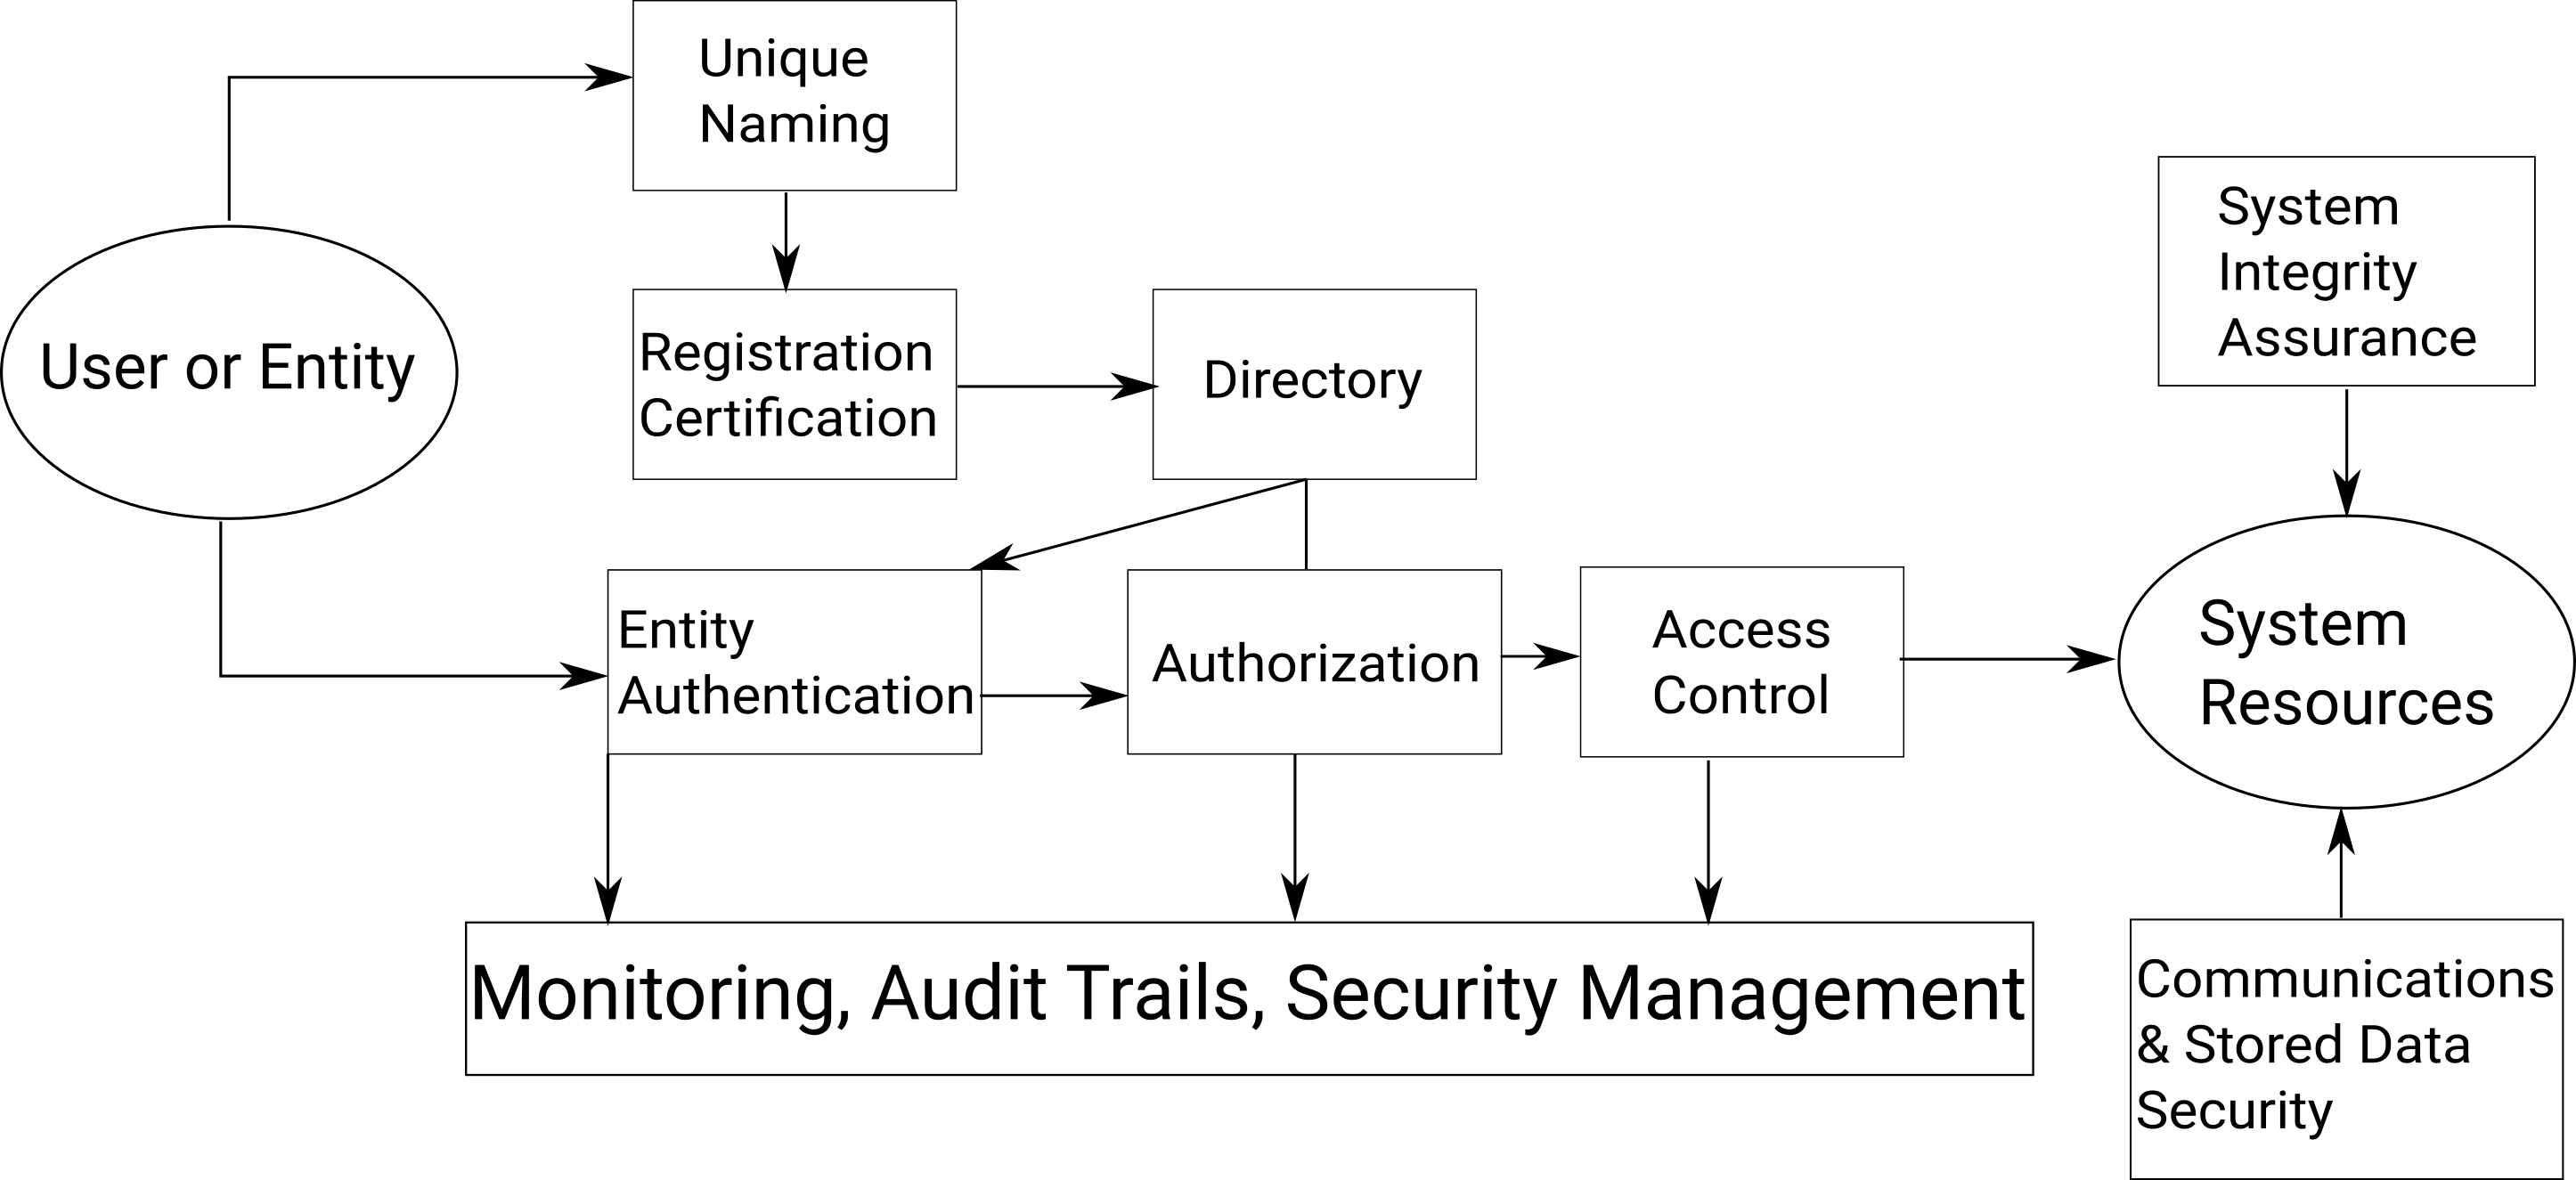
\includegraphics[scale=0.5]{./Drawings/EITP20-Secure_Systems_Engineering/Major_Security_Services_Relations.png}
  \end{solution}

  \begin{parts}
  \part{} Describe each of the different steps
  \part{} What is the end result?
  \part{} Give an example of a logical security architecture
  \end{parts}

\item What is a physical security architecture?
\item A physical security architecture when using the SABSA include making a mapping to physical security mechanisms
  \begin{parts}
  \part{} Describe what is meant by a ``Naming and registration'' mechanism and give examples
  \part{} Describe what is meant by a ``Storage and runtime'' mechanism and give examples
  \part{} Describe what is meant by a ``Physical security'' mechanism and give examples
  \part{} Describe what is meant by an ``Authentication and session'' protection mechanism and give examples
  \part{} Describe what is meant by a ``User interface and naming'' mechanism and give examples
  \part{} Describe what is meant by a ``Authorization and access control'' mechanism and give examples
  \part{} Describe what is meant by a ``Monitoring and incident'' mechanism and give examples
  \end{parts}

\item What must in addition to the security mechanisms be specified in the physical security architecture?
\item Give example of platform security solution that can be used to build solutions meeting a logical security services and can be used to protect the chosen physical security mechanism?
\item For the SSO logical security architecture given at the lecture, perform the following:
  \begin{parts}
  \part{} Identify the main physical security mechanisms needed in the corresponding physical security architecture.
  \part{} Identify the main platform security components needed to fulfil the architecture
    \begin{subparts}
    \subpart{} Suggest concrete platform security mechanisms to use for the physical realization.
    \end{subparts}
  \end{parts}
\end{questions}

%%% Local Variables:
%%% mode: latex
%%% TeX-master: "../EITP20-Secure_Systems_Engineering-Study_Questions"
%%% End:
